 \item Dodanie części - scenariusz główny \\
 
 Opis słowny - ten przypadek użycia opisuje funkcjonalność dodawania nowych typów części, czyli takich które nie są jeszcze zarejestrowane w systemie. Obejmuje to sytuację, gdy np. sklep decyduje się na wprowadzenie nowego asortymentu do sprzedaży.
 
 \begin{longtable}{|p{5cm}|p{7cm}|}
 	\hline
	\textbf{Aktor} & Pracownik \\
	\hline
	\textbf{Warunki początkowe} & Posiadanie konta z uprawnieniami umożliwiającymi zarządzanie częściami, zalogowanie się do systemu \\
	\hline
	\textbf{Opis przebiegu interakcji} & Wybór prezentacji listy części na stronie głównej sklepu, wybranie opcji dodania nowej części, uzupełnienie danych, zatwierdzenie operacji \\
	\hline
	\textbf{Sytuacje wyjątkowe} & Dodawana część już istnieje, podanie błędnych danych nowej części \\
	\hline
	\textbf{Warunki końcowe} & Dodanie do systemu nowego typu części \\
	\hline
 \end{longtable}
 
  \item Dodanie części - scenariusz główny \\
  \begin{tabularx}{\linewidth}{ c X}
  Aktor: & Pracownik \\
  \end{tabularx}
   \begin{enumerate}
    \item Scenariusz ``Wyświetlanie listy części - scenariusz alternatywny - użytkownik posiada specjalne uprawnienia do zarządzania częściami''. \label{dodanie-czesci-poczatek}
    \item Pracownik wybiera opcję dodania nowej części.
    \item System prezentuje pracownikowi formatkę dodania nowej części, z możliwością wypełnienia następujących atrybutów części:
    \begin{enumerate}
      \item Kod części (generowany automatycznie, z możliwością edycji przez pracownika)
      \item Nazwa części
      \item Opis części
      \item Zdjęcie części (w jedym z popularnych formatów graficznych, takich jak JPG, PNG czy GIF)
      \item Cena jednostkowa części
      \item Widoczność części dla klientów (czy klienci będą mogli zobaczyć część na liście części możliwych do kupienia)
      \item Minimalna liczba sztuk w magazynie
    \end{enumerate}
    \item Pracownik uzupełnia wymagane pola i zatwierdza operację. \label{dodanie-czesci-zatwierdzenie}
    \item System dodaje część do bazy danych i informuje użytkownika o zakończeniu operacji.
  \end{enumerate}
  
  \item Dodanie części - scenariusz alternatywny - dodawana część już istnieje \\
  \begin{tabularx}{\linewidth}{ c X}
  Aktor: & Pracownik \\
  \end{tabularx}
   \begin{enumerate}
    \item Kroki \ref{dodanie-czesci-poczatek} do \ref{dodanie-czesci-zatwierdzenie} scenariusza głównego.
    \item System sprawdza czy istnieje już część o podanym kodzie. Jeśli tak, wyświetla komunikat o błędzie i anuluje operację. Jeśli nie, to powrót do scenariusza głównego.
  \end{enumerate}
  
  \item Dodanie części - scenariusz alternatywny - podanie błędnych danych nowej części \\
  \begin{tabularx}{\linewidth}{ c X}
  Aktor: & Pracownik \\
  \end{tabularx}
   \begin{enumerate}
    \item Kroki \ref{dodanie-czesci-poczatek} do \ref{dodanie-czesci-zatwierdzenie} scenariusza głównego.
    \item System sprawdza czy podane przez użytkownika dane są poprawne, czyli:
    \begin{enumerate}
      \item Czy wszystkie pola oprócz opisu i zdjęcia są wypełnione
      \item Czy podana cena nie jest ujemna
      \item Czy podana minimalna liczba sztuk na magazynie nie jest ujemna
    \end{enumerate}
    \item W przypadku niepoprawności wprowadzonych danych, system wyświetla stosowny komunikat błędu i anuluje operację. W przeciwnym przypadku powrót do scenariusza głównego.
  \end{enumerate}
  	
\begin{figure}[h!]
    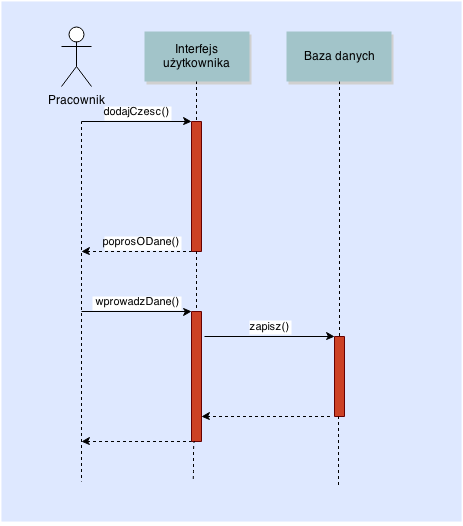
\includegraphics[width=\textwidth,
    height=0.7\textheight]{graphics/UseCase/Czesci/DodanieCzesciSD.png}
  \caption{Diagram sekwencji dla przypadku użycia Dodanie części - scenariusz główny}
\end{figure}